\documentclass[11pt]{article}
\usepackage{graphicx}
\usepackage{geometry}
\usepackage{hyperref}
\usepackage[utf8x]{inputenc}
\usepackage{wrapfig}

\usepackage{xcolor}  % temporary, for TODO's

\title{BETH 2019: Report MinusMinusEnergy}
\author{Marie-Louise Achart, Matthias Busenhart, Yannick Niedermayr,\\Philip Wiese, Manuel Winkler}
\date{\today}

\begin{document}

\maketitle

\section{Introduction}
This report is part of the ETH: Blockchain School for Sustainability, which took place in February 11-15, 2019, at ETH Zurich. More information about this week can be found at: \hyperref[www.beth.ethz.ch]{www.beth.ethz.ch}.\\
We worked during the Hackathon on the challenge presented by Energy Switzerland:\\ \textit{How could Blockchain technology benefit the climate twice with a solution that documents:\\
1) CO$_2$ emission reduction by households\\
2) The reinvestment of saved costs in (local) sustainable projects with direct payments},\\
with the requirement to provide a solution as energy efficient as possible.\\
We first will do a literature review of the different aspects of the blockchain technology that could be relevant for this challenge. Then we will present our solution's concept, implementation and evaluation. Finally we will discuss further developments and alternatives.\\

\section{Literature Review}
Explained by Satoshi Nakamoto in 2008, with a paper about Bitcoin, the blockchain is grounded on two technologies: asymmetric cryptography and distributed systems. There are already a substantial number of blockchain-based applications related to diverse fields such as finance, integrity verification, governance, citizenship, user services, public sector, voting, Internet of Things (IoT), healthcare management, privacy and security, business and industry, supply chain, energy sector, education and data management.\cite{1} \\
The well-known Bitcoin is just one use case of the blockchain technology. There is a whole world beyond cryptocurrencies that could benefit from the unique confluence of smart contracts and smart devices.\\\\
Smart contracts are user-defined programs or protocols that can be automatically enforced once certain preconditions are met. Those executable programs define rules for writing in the distributed ledger, without the need of any centralized control. Building trust in a distributed environment will change the way we share information, interact with each other and thus do business, especially in the IoT industry.\cite{2}\\\\
As shown in figure \ref{img_state} on page \pageref{img_state}, the number of electronic devices around us is always growing, with already more than seven billion IoT devices in 2018. A large part of the future growth should come from low-power wide area networtk (LPWAN), a technology allowing an extremely high battery life and a maximum communication range over 20 kilometers. There is already more than 25 Millions devices - the majority of which are smart meters - connected through LPWAN, and this number should increase to more than two billion devices by 2025.\\

\begin{figure}
	\begin{center}
		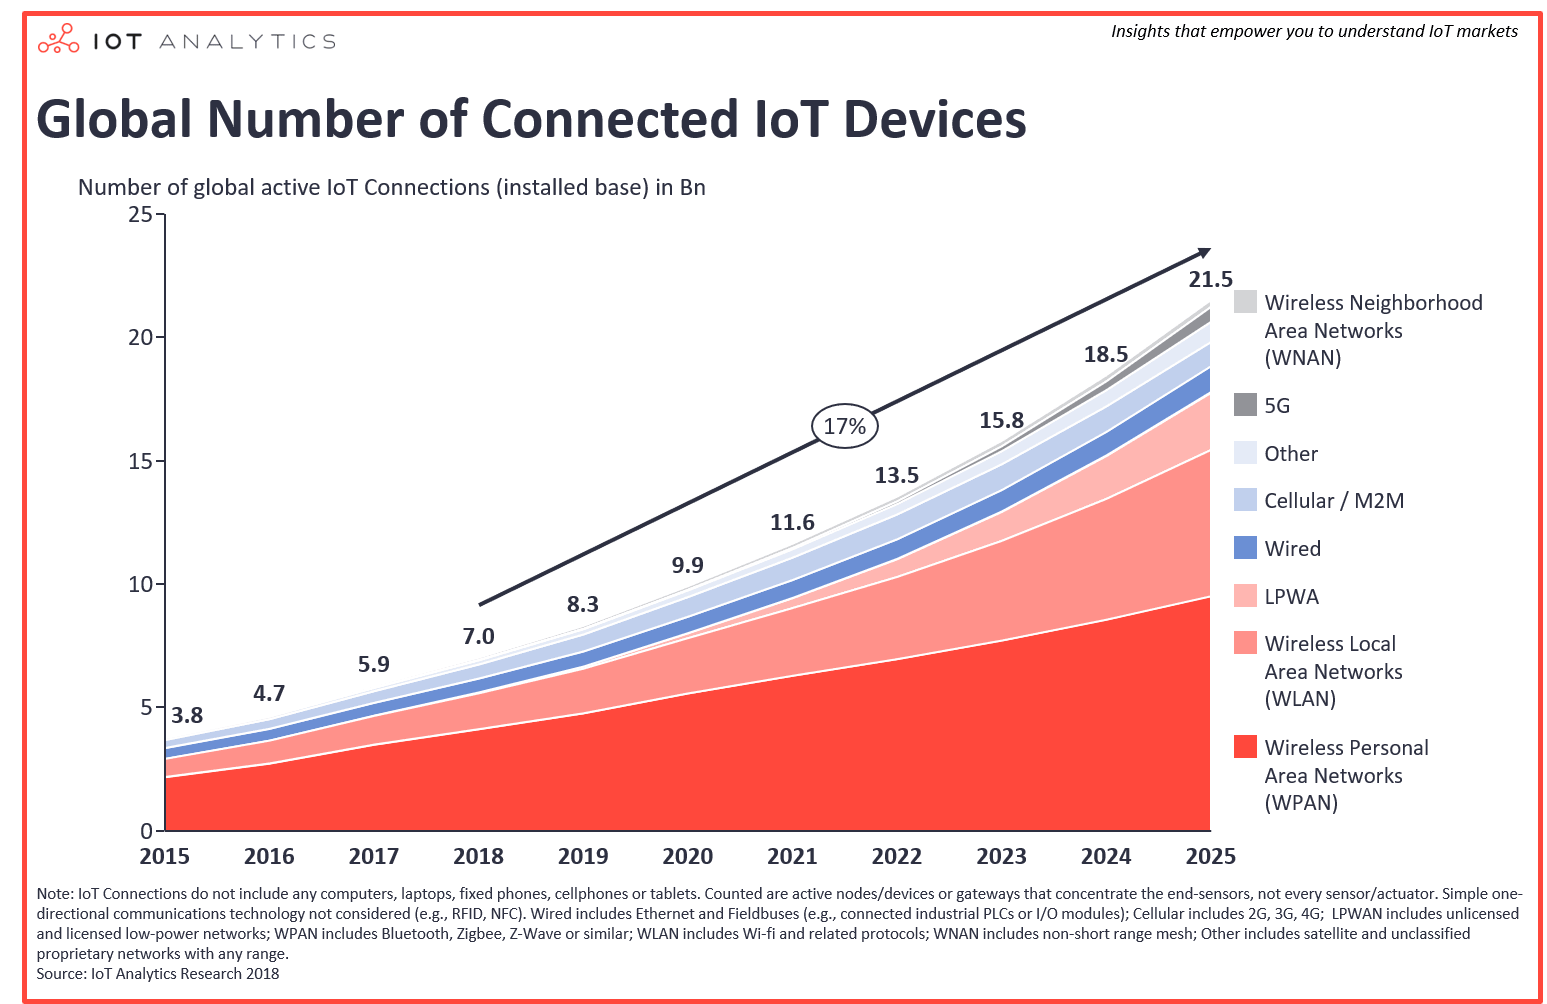
\includegraphics[scale=0.275]{stateofIoT2018.png}
		\caption{State of IoT 2018, \cite{3}}
		\label{img_state}
	\end{center}
\end{figure}

Smart meters allows to monitor electric energy consumption. This data can then be transmitted to energy suppliers for billing. Although a large amount of data provided by smart devices - like the ones recorded by smart meters - could be used to adequately adjust energy consumption and/or optimize networks, it may also raise critical privacy issues \cite{4} that the blockchain technology can potentially solve.\\
Generally, the specificities of the energy sector could enable major transformations thanks to blockchain technology. Indeed it is characterized by millions of transactions to trade and distribute energy that trusted payments systems built on a blockchain could automate. Furthermore, the existing grids could be optimized based on more data control at the facilities level using a decentralized platform. The potential impact could be of a massive scale, reaching millions of users currently connected by the regular grid. Although for more than half of the blockchain initiatives related to energy, climate and the environment, the time frame for impact is two or more years, due to the necessity to negotiate and partner with utility companies.\cite{5}\\\\
When facing the energy waste issue, monitoring in real time could potentially save 4 650 TWh in 2040, far more than their expected cost of 275 TWh for that same year. Active tracking and predicting the energy performance of buildings would help to reduce peak loads, and control that energy is really consumed when and where it is needed. Useful insights from this data would enhance power system performance and asset diagnostics which can lead to cost reduction when e.g. investments are not performing as expected or when maintenance is needed. Thus energy savings - achieved at a limited energy cost - could benefit consumers.\cite{6}\\\\
At the moment there are no suitable solutions for consumers to manage their energy supply either with some active control or with an automated software. What could really affect the energy sector will not be a small group of consumers using blockchain applications in small decentralized networks, but effective and easy to use applications and software reaching the majority of consumers. Without those user-friendly applications and/or automated software (e.g. using learning algorithms that automatically program heating and cooling services) that are used on a large scale, the blockchain technology will not affect the energy sector in a noticeable manner.\cite{7}\\\\
There are two major challenges to overcome if we want the Internet of Things to be widely accepted and adopted: the lack of standardization and trust issues. The actual heterogeneity in the field, resulting from the huge expansion of the IoT, needs to be lessened with the help of standard mechanisms and protocols. Regarding the trust issue, the blockchain technology could provide a reasonable answer. The threat that untrusted entities alter information according to their own interests can no longer exist if all participants are part of a distributed system where the data is owned by everyone, is easy to verify, and remains immutable. The development of cloud computing did stimulate the IoT applications, but it is characterized by a centralized architecture that does not provide reliable traceability to ensure enough trust among the network participants. Data transparency is a key for the further adoption of IoT.\cite{21}\\\\
One of the main leverage to reduce energy consumption lies in the residential sector. Adopting a Home Automation System (HAS): a smart home system that combines Wireless Sensor and Actuator Networks (WSAN) with Computational Intelligence technique could be a way to address this issue.\cite{15}\\\\
Blockchains enable digital peer-to-peer transactions, thus could facilitate machine-to-machine communication and data transfers between smart devices. Digitalisation and IoT platforms promise to improve network efficiency, billing processes and supply chain, offering the opportunity to optimize demand aggregation services and demand response, and lowering management costs with remote maintenance and control.\cite{8}\\
Indeed the Internet of Things became the main standard for low-power lossy networks (LLN) having constrained ressources, where embedded devices having sensors are interconnected. Those devices' wide acceptance and popularity are the result of the rapid growth in miniaturization, electronics and wireless communication technologies, e.g. adding cognitive radio based networks to the underutilized frequency spectrum to improve bandwidth.\cite{9}\\\\
The further development of the components of blockchain-based energy systems, like smartphone apps, sensor technologies, smart devices, smart homes, etc. will allow smart grids to blossom. In this new vision, interconnected smart devices coordinate and adjust their power consumption to price, availability or grid stability signals. To reach this state with a large number of devices producing high volume of data at high frequency, a centralized approach becomes inefficient. Thus, local decision-making and distributed control is more suitable. They help to lower the consumption of the computational ressources needed to optimally operate power systems.\cite{8}\\
Assuring interoperability in smart grids and IoT applications, the blockchain technology could improve competition between energy suppliers, by providing better felxibility to consumers. They could switch more easily from one energy supplier to another, as the energy market operations could become more efficient and more transparent.\cite{20}\\\\
Pursuing energy efficiency became a goal for many governments and institutions. There is no one and only appropriate solution to deal with this issue. Policies that apply a more diverse and flexible approach seem more successful. The example of New Zealand, a renewable-rich country could be inspiring for Switzerland, where only 62\% of consumed electricity comes from renewable sources\cite{10}. The recommendations for New Zealand include: raising consumer awareness, public procurement, developing strong measurement and verification systems, revisiting the housing energy efficiency strategies and promoting the energy efficiency research and product development. \{\color{red} DID: I tried to rewrite it... Feel free to revert, I don't know if I even got the meaning right. \color{black}\}    One important step of implementing those beneficial policies is to make the citizens adhere to their improvements in dealing with urgent environmental issues. As stated in the same paper, displaying well-designed awareness programs in form of television commercials that reached 69\% of New Zealanders, motivated 40\% to take actions to reduce their energy consumption. \cite{11}\\\\
Besides the traditional television commercials, there are many other ways to create incentives for citizens to act appropriately regarding environmental agendas. The example of \#SmartME which provides a virtual complementary currency for access and payments of registered services within a bigger ecosystem, including university cafeterias, etc. The \#SmartME incentive mechanism is implemented through an Android-based mobile app. This concept could be a first step toward smart cities. Indeed blockchain could be a good candidate to turn the smart city concept into reality, since it would enable devices to be more autonomous with easier exchange of trusted information recorded on a distributed open ledger.\cite{12}\\\\
Another paper presented the reasons why people adopt certain environmental-friendly behaviors related to waste, reusing and recycling. It emerged that both strong belief in an intrinsic value in nature and convenience-based factors were important to enhance actual behaviors. It underlies the importance to design easy to use and convenient ways to reduce energy consumption until those new behaviors become a norm widely accepted among citizens. Efforts to further raise awareness of environmental issues will definitely help to reshape fundamental values of the consumers, but it should go in pair with a more practical approach.\cite{13}\\\\
There are 3 agendas that could support smart urban development: more control and optimization of urban infrastructure with embedded digital technology, more analysis of the datasets produced in the smart cities using big data and more citizen participation with digitally-enabled democratic decision-making in urban governance. A good implementation is the Better Reykjavik platform, where citizens can submit and vote for projects funded by the municipality.\cite{14}\\\\
To reach an intelligent energy management, the utilization of cross-domain data could support the creation, development, maintenance and exploitation of smart energy services. This shift from data scarcity to data abundance could be done with some big data platform that authorities and local administrations, energy service companies, energy managers and consultants, energy providers could access.\cite{17}\cite{19}\\\\
The benefits following from a systematic use of large chunk of data, like more effective policies and regulation of techno-socio-economic systems supported by IoT technologies must be balanced against the need for privacy protection. Indeed surveillance and discriminatory actions leading to segregation phenomena could ensue from large-scale access to consumer data. An interesting alternative to this dilemma is a supply-demand system run by computational markets. On one hand the citizen is incentivized, but can decide which level of information he wants to share. On the other hand data aggregators reward citizens that give them the data to realize accurate computing analytics required for more informed decision-making.\cite{18}\\\\
Not only the cities can affected by the rapidly emerging embedded intelligence, the agriculture could also benefit from this transformative approach. For a further analysis of smart agriculture, you can refer to this paper\cite{16}.\\\\
Even if the emergence of new ideas and the implementation of pilot projects results from a bottom-up approach, the government has a major role to play to facilitate the funding of those renewable energy projects in most stages, especially via government policies and building an appropriate regulatory environment. Sustainable projects are still heavily dependent on the support a state can provide, often in the form of subsidies, differential feed-in-tariffs (compared with conventional power tariffs), or regulatory arrangements (such as carbon trading).\cite{22}\\

\section{Presentation of our solution (4pages)}

\color{red} TODO: why disruptive solution? \color{black}
\subsection{Solution Concept}
To design a realistic and working solution to the given challenge by SwissEnergy some boundary conditions had first to be defined. We assumed that
\begin{enumerate}\itemsep0pt
	\item There is a subsidising party (e.g. government, NGO\footnote{Non-governmental organization})
	\item The local energy producer can be trusted
	\item The end consumer are not able to physically manipulate the smart meters
\end{enumerate}

The basic idea of our solution consists on the concept that the end consumer (client) is rewarded for an energy consumption below a defined target. This target has to be defined by the subsisizing party based on the wanted consumption reduction and the amount of available subsidies. The client is able to claim MME tokens for his consumption reduction and use the tokens to pay part of his bill and/or invest the tokens into the fond. In the future, the fond can be extended voting system to reinvest the saved assest into local or global sustainable projects.

\newpage
\subsubsection{Example}
\begin{wraptable}{r}{4cm}
\begin{tabular}{ll}
\multicolumn{2}{c}{\textbf{Parameter}}                                                                                                                 \\ \hline
CHF / kWh\footnote{\href{https://www.swissgrid.ch/en/home/customers/topics/tariffs.html}{Swissgrid Tarifs}} & 0.19 \\ \hline
g CO2 / kWh                                                                                                                                     & 29.8 \\ \hline
MME / kg CO2                                                                                                                                    & 700  \\ \hline
CHF / MME                                                                                                                                       & 0.01
\end{tabular}
\label{table_parameter}
\end{wraptable}
A swiss houshold in a one-familiy house with 4 persons consumes at average 5200  kWh per year.\footnote{\href{https://www.bundespublikationen.admin.ch/cshop_mimes_bbl/2C/2C59E545D7371ED5BB89418480F1B62D.pdf}{Bundespublikationen: 805.902.D}} The government defines a target reduction of 10\% of the average energy consumption and subidies at maximum of 120.- CHF per houshold. \\\\
A sample end consumer uses 4940 kWh in one year wich is 5\% below the average. This values are generated by a smart meter installed by the energy provider. The data is send regularly to a client server to analyze and visualize the energy consumption for the end consumer. On a monthly basiss the sensor data is used to claim token for the reduced energy consumption.

\begin{table}[ht]
\begin{tabular}{ll|llllll|lll}
\textbf{Reduction} & \textbf{} & \textbf{Consumption} & \textbf{Costs} & \textbf{Reduction} & \textbf{CO2} & \textbf{Reward} &           \\
                   &           & {[}kWh{]}            & {[}CHF{]}      & {[}kWh{]}          & {[}kg{]}     & {[}MME{]}       & {[}CHF{]} \\ \hline
Target             & 10\%      & 4680                 & 889            & 520                & 15.5         & 10847           & 108       \\
Actual             & 5\%       & 4940                 & 939            & 260                & 7.7          & 5424            & 54
\end{tabular}
\caption{Reduction target and actual reduction reward}
\label{table_target-actual}
\end{table}

\begin{figure}[ht]
	\begin{center}
		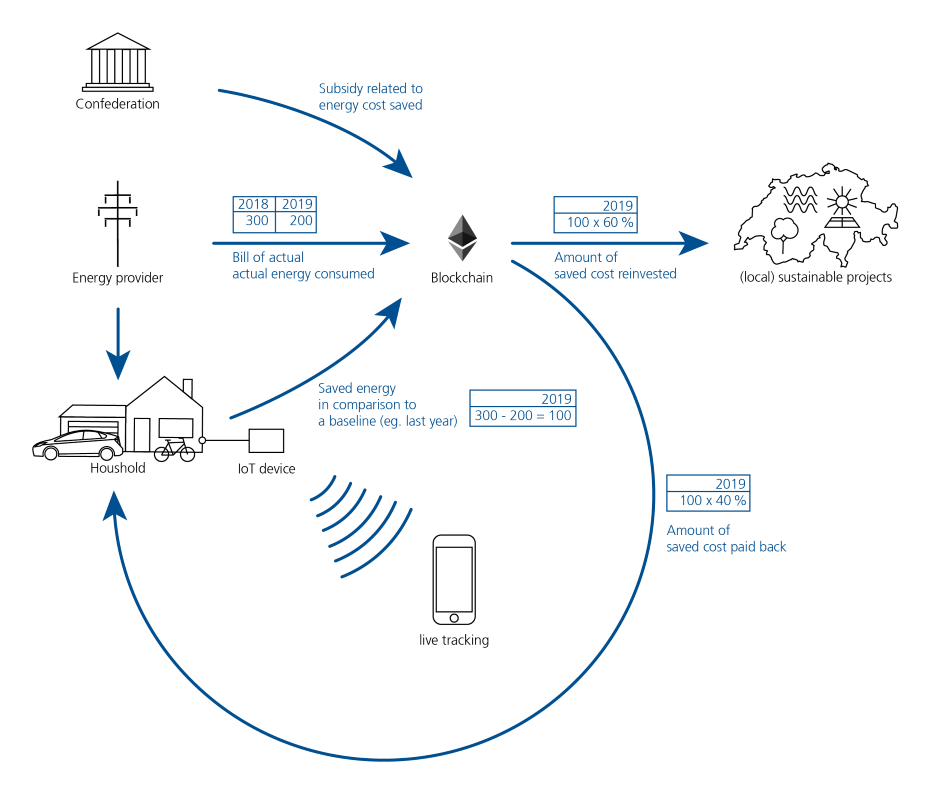
\includegraphics[scale=1.5]{concept.png}
		\caption{Our concept}
		\label{img_concept}
	\end{center}
\end{figure}


\subsection{Solution Design}
\subsubsection{Architecture}
For the BETH-Event, we created individual modules, each will be discussed later. A small overview is presented in figure \ref{img_impl} on page \pageref{img_impl}.\\\\
Ethereum is a decentralized platform that runs smart contracts. These apps (smart contracts) run on a custom built blockchain, an enormously powerful shared global infrastructure that can move value around and represent the ownership of property.\cite{23}



\subsubsection{Smart Contracts}
The smart contracts on the \hyperref[https://www.ethereum.org/]{Ethereum}\footnote{\href{https://www.ethereum.org/}{https://www.ethereum.org/}} blockchain were implemented in the high-level programming language Solidity. The ownership of these contracts belongs ideally to the subsidizing party e.g. the government.
We separated the functionality into three different contracts.
\begin{figure}[ht]
	\begin{center}
		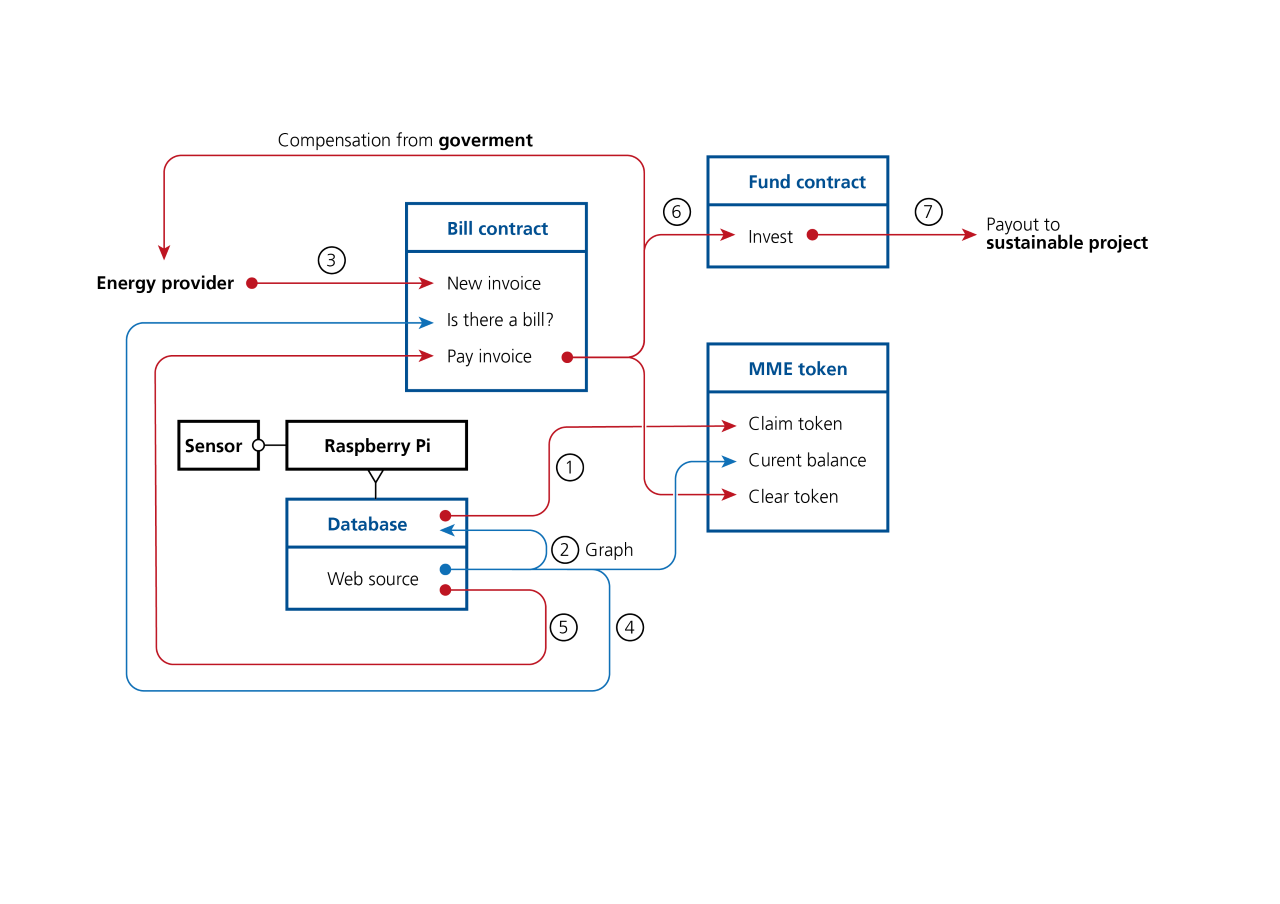
\includegraphics[scale=1.5]{implementation.png}
		\caption{Our implementation}
		\label{img_impl}
	\end{center}
\end{figure}

\paragraph{MME Token Contract}
The MME contract is a ERC20\footnote{https://eips.ethereum.org/EIPS/eip-20} compliant token contract. It manages the token balance of addresses and allows to claim new token in exchange for the proof of energy consumption reduction. \\\\

The sensor data is cryptographically signed using elliptic curve cryptography (ECC)\cite{24} inside the sensor and then send to the MME contract. The contract validates the signature of the data and also prevents replay attacks.\footnote{A replay attack is a form of network attack in which a valid data transmission is maliciously or fraudulently. repeated.}
\paragraph{Bill Contract}
The bill contract handles the creation of invoices for clients by the energy providers and the payment of these. The currency of the invoices is ether. The owner of the contract is able to add new invoice issuer. When a payment is made to the bill contract the client includes the desired ratio of available tokens to use for a reduction of his invoice.
\paragraph{Fund Contract}
Test\\



\subsubsection{IoT-Sensor}
We envisioned the system to use an IoT Sensor that measures energy consumption, a smart meter. This measured data (preferably given in kilowatt hours or similar) would be used to track the consumption reduction progress of a consumer from cycle to cycle. \\
Since we did not have such a sensor, the github code from the Hackathon uses a light sensor that provides analog data and is simply used as a proof of concept.

\subsubsection{Broker}
The data broker consists of two components. \\
Firstly, we have a python script\footnote{src/client/broker/sensorDataHandler.py} that simply extracts sensor data values and writes them to a SQLite3 database. \\
For our system to work properly it is a requirement for the sensor to add a signature to the data that is later verified by the contract. This signing process must be so hard to reverse-engineer that one cannot generate any profit out of simply breaking the sensor open and extracting a private key.
The data handler is what we call a C++ program\footnote{src/client/broker/datahandler.cpp} that is used to determine how much energy a consumer has saved in a cycle. The program first extracts the energy consumption in the current cycle from the SQLite3 database. Afterwards, it creates a signed transaction from the extracted data and sends them to the MMEToken contract on the blockchain.\\
A relatively small problem that however we have yet to solve is performance-related: The calculation step of the tokens can be non-trivial, especially if the evaluation of the statistics should be as fair as possible i.e. taking into account the number of persons consuming power that passes through this sensor, the heating system of the house and many more similar factors. These small calculations eventually pile up to a very large amount of computation power ?expended? by the blockchain that possibly could be saved by moving this calculation onto a small computer
that is built into the sensor casing. This would however open up another possibility for fraudsters to exploit the system by hijacking this computer.

\subsubsection{Webserver}
Our webserver runs with NodeJS\footnote{https://nodejs.org}. It connects to the database created by the Broker and serves a frontpage with the data shown in a graph. The user can select two distinct dates and view his energy consumption between those dates. In the navigation menu, the user can go to the bill page, where, if he received an invoice, he can choose how many of his tokens he will spend for lowering his bill and how many should go to the fond. At last, he can submit his payment via MetaMask. The backend of the server runs a simple javascript-file, namely app.js\footnote{src/client/webserver/app.js}. It loads from the config-file several values (i.e. contract address, wallet address, and more). This data will be used for connecting to the contract on the Ethereum blockchain and later for checking if the user has a new invoice to pay. The frontend of the page is written in the template engine \hyperref[https://pugjs.org]{PugJS}\footnote{https://pugjs.org}. The pages are served with routes from the backend node server.

\subsection{Code abstracts}
\color{red} TODO: Everyone? \color{black}

\subsection{our solution evaluation: features, bugs...}
blockchain for social impact: methodology from \textit{Stanford Business School, Center for Social Innovation, 2018, Blockchain For Social Impact Moving Beyond The Hype}:\\
1-what is the problem of your organization is trying to solve? What are your end users?\\
2-How does your initiative use blockchain, and why is blockchain a good technology for this problem?\\
3-What technologies or services are available to solve this problem, and how is blockchain a better solution?\\
4-what is your initiative's intended impact? How do you measure it?\\
5-In what time do you think you will see meaningful impact from your blockchain initiative?\\

\section{Conclusion}
\color{red} TODO \color{black}

\begin{thebibliography}{22}

\bibitem{1}
	Fran Casino, Thomas K.\,Dasaklis, Constantinos Patsakis,
	\textit{A systematic literature review of blockchain-based applications: Current status, classification and open issues},
	\hyperref[https://doi.org/10.1016/j.tele.2018.11.006]{https://doi.org/10.1016/j.tele.2018.11.006}
\bibitem{2}
	Ana Reyna, Cristian Martín, Jaime Chen, Enrique Soler, Manuel Díaz,\\
	\textit{On blockchain and its integration with IoT. Challenges and opportunities}\\
	\hyperref[https://doi.org/10.1016/j.future.2018.05.046]{https://doi.org/10.1016/j.future.2018.05.046}
\bibitem{3}
	Knud Lasse Lueth,\\
	\textit{State of the IoT 2018: Number of IoT devices now at 7B – Market accelerating}\\
	\hyperref[https://iot-analytics.com/state-of-the-iot-update-q1-q2-2018-number-of-iot-devices-now-7b/]{https://iot-analytics.com/state-of-the-iot-update-q1-q2-2018-number-of-iot-devices-now-7b/}
\bibitem{4}
	Marco Conoscenti, Antonio Vetrò, Juan Carlos De Martin,\\
	\textit{Blockchain for the Internet of Things: a Systematic Literature Review}\\
	\hyperref[https://ieeexplore.ieee.org/abstract/document/7945805]{https://ieeexplore.ieee.org/abstract/document/7945805}
\bibitem{5}
	Doug Galen, Nikki Brand, Lyndsey Boucherle, Rose Davis, Natalie Do, Ben El-Baz, Isadora Kimura, Kate Wharton, Jay Lee,\\
	\textit{Blockchain for social impact. Moving beyond the hype}\\
	\hyperref[https://www.gsb.stanford.edu/sites/gsb/files/publication-pdf/study-blockchain-impact-moving-beyond-hype_0.pdf]{https://www.gsb.stanford.edu/sites/gsb/files/publication-pdf/study-blockchain-impact-moving-beyond-hype\_0.pdf}
\bibitem{6}
	International Energy Agency,\\
	\textit{Digitalization \& Energy}\\
	\hyperref[https://www.iea.org/publications/freepublications/publication/DigitalizationandEnergy3.pdf]{https://www.iea.org/publications/freepublications/publication/DigitalizationandEnergy3.pdf}
\bibitem{7}
	PwC global power \& utilities\\
	\textit{Blockchain – an opportunity for energy producers and consumers?}\\
	\hyperref[https://www.pwc.com/gx/en/industries/assets/pwc-blockchain-opportunity-for-energy-producers-and-consumers.pdf]{https://www.pwc.com/gx/en/industries/assets/pwc-blockchain-opportunity-for-energy-producers-and-consumers.pdf}
\bibitem{8}
	Merlinda Andoni, Valentin Robu, David Flynn, Simone Abram, Dale Geach,  David Jenkins, Peter McCallum, Andrew Peacock,\\
	\textit{Blockchain technology in the energy sector: A systematic review of challenges and opportunities}\\
	\hyperref[https://doi.org/10.1016/j.rser.2018.10.014]{https://doi.org/10.1016/j.rser.2018.10.014}
\bibitem{9}
	Minhaj Ahmad Khan, Khaled Salah, \\
	\textit{IoT security: Review, blockchain solutions, and open challenges}\\
	\hyperref[https://doi.org/10.1016/j.future.2017.11.022]{https://doi.org/10.1016/j.future.2017.11.022}
\bibitem{10}
	Office federal de l'energie OFEN, \\
	\hyperref[https://www.newsd.admin.ch/newsd/message/attachments/51791.pdf]{https://www.newsd.admin.ch/newsd/message/attachments/51791.pdf}\\
	\hyperref[http://www.bfe.admin.ch/energie]{http://www.bfe.admin.ch/energie}
\bibitem{11}
	Piyush Verma, Nitish Patel, Nirmal-Kumar C. Nair, Alan C. Brent, \\
	\textit{Improving the energy efficiency of the New Zealand economy: A policy comparison with other renewable-rich countries}\\
	\hyperref[https://doi.org/10.1016/j.enpol.2018.08.002]{https://doi.org/10.1016/j.enpol.2018.08.002}
\bibitem{12}
	Dario Bruneo, Salvatore Distefano, Maurizio Giacobbe, Antonino Longo Minnolo, Francesco Longo, Giovanni Merlino, Davide Mulfari, Alfonso Panarello, Giuseppe Patanè, Antonio Puliafito, Carlo Puliafito, Nachiket Tapas, \\
	\textit{An IoT service ecosystem for Smart Cities: The \#SmartME project}\\
	\hyperref[https://doi.org/10.1016/j.iot.2018.11.004]{https://doi.org/10.1016/j.iot.2018.11.004}
\bibitem{13}
	Stewart Barr, \\
	\textit{Factors Influencing Environmental Attitudes and Behaviors. A U.K. Case Study of Household Waste Management}\\
	\hyperref[https://doi.org/10.1177/0013916505283421]{https://doi.org/10.1177/0013916505283421}
\bibitem{14}
	Christopher Martin, James Evans, Andrew Karvonen, Dujuan Yang, Trond Linjordet, \\
	\textit{Smart-sustainability: A new urban fix?}\\
	\hyperref[https://doi.org/10.1016/j.scs.2018.11.028]{https://doi.org/10.1016/j.scs.2018.11.028}
\bibitem{15}
	Geraldo P.R. Filho, Leandro A. Villas, Vinícius P. Gonçalves, Gustavo Pessin, Antonio A.F. Loureiro, Jó Ueyama, \\
	\textit{Energy-efficient smart home systems: Infrastructure
		and decision-making process}\\
	\hyperref[https://doi.org/10.1016/j.iot.2018.12.004]{https://doi.org/10.1016/j.iot.2018.12.004}
\bibitem{16}
	Wu Yong, Li Shuaishuai, Li Li, Li Minzan, Li Ming, K.G. Arvanitis, Cs. Georgieva, N. Sigrimis, \\
	\textit{Smart Sensors from Ground to cloud and Web Intelligence}\\
	\hyperref[https://www.sciencedirect.com/science/article/pii/S240589631831173X]{https://www.sciencedirect.com/science/article/pii/S240589631831173X}
\bibitem{17}
	Francis G.N. Li, Chris Bataille, Steve Pye, Aidan O'Sullivan, \\
	\textit{Prospects for energy economy modelling with big data: Hype, eliminating blind spots, or revolutionising the state of the art?}\\
	\hyperref[https://doi.org/10.1016/j.apenergy.2019.02.002]{https://doi.org/10.1016/j.apenergy.2019.02.002}
\bibitem{18}
	Pournaras Evangelos, Nikolic Jovan, Velásquez Pablo, Trovati Marcello, Bessis Nik, Helbing Dirk, \\
	\textit{Self-regulatory information sharing in participatory social sensing}\\
	\hyperref[https://www.researchgate.net/publication/299550923_Self-regulatory_information_sharing_in_participatory_social_sensing]{https://www.researchgate.net/publication/299550923\_Self-regulatory\_information\_sharing\_in\_participatory\_social\_sensing}
\bibitem{19}
	Vangelis Marinakis, Haris Doukas, John Tsapelas, Spyros Mouzakitis, Álvaro Sicilia, Leandro Madrazo, Sgouris Sgouridis, \\
	\textit{From big data to smart energy services: An application for intelligent energy management}\\
	\hyperref[https://doi.org/10.1016/j.future.2018.04.062]{https://doi.org/10.1016/j.future.2018.04.062}
\bibitem{20}
	Grewal-Carr V, Marshall S., \\
	\textit{Blockchain enigma paradox opportunity.}\\
	\hyperref[https://www2.deloitte.com/content/dam/Deloitte/uk/Documents/Innovation/deloitte-uk-blockchain-full-report.pdf]{https://www2.deloitte.com/content/dam/Deloitte/uk/Documents/Innovation/deloitte-uk-blockchain-full-report.pdf}
\bibitem{21}
	Ana Reyna, Cristian Martín, Jaime Chen, Enrique Soler, Manuel Díaz, \\
	\textit{On blockchain and its integration with IoT. Challenges and opportunities.}\\
	\hyperref[https://doi.org/10.1016/j.future.2018.05.046]{https://doi.org/10.1016/j.future.2018.05.046}
\bibitem{22}
	Patrick T.I. Lam, Angel O.K. Law, \\
	\textit{Financing for renewable energy projects: A decision guide by developmental stages with case studies}\\
	\hyperref[https://doi.org/10.1016/j.rser.2018.03.083]{https://doi.org/10.1016/j.rser.2018.03.083}
\bibitem{23}
	Vitalik Buterin, \\
	\textit{Ethereum: A Next-Generation Smart
Contract and Decentralized Application Platform.}\\
	\hyperref[https://www.ethereum.org/]{https://www.ethereum.org/}  (visited on 23.02.2018)
\bibitem{24}
	V. S. Miller, \\
	\textit{Use of elliptic curves in cryptography. In H. C. Williams, editor, CRYPTO, volume 218 of
LNCS,}\\
	  pages 417–426. Springer, 1986.




\end{thebibliography}


\end{document}
